\documentclass[../main/main.tex]{subfiles}
\begin{document}

\dominitoc
\faketableofcontents
\dominilof
\fakelistoffigures
\dominilot
\fakelistoftables

\chapter{Introduction \`a \snana}\label{ch:snana}
\epigraph{\openquote\textit{A common mistake that people make when trying to
design something completely foolproof is to underestimate the ingenuity of
complete fools}\closequote}{Douglas \textsc{Adams}, \textit{Mostly Harmless}}

Nous avons vu Chapitre~\ref{ch:sne} qu'à partir de 1993, grâce la
standardisation des SNe~Ia par l'étude de leurs caractéristiques d'étirement et
de couleur notamment, la cosmologie basée sur les SNe~Ia a pu prospérer, donnant
une incertitude sur les modules de distances d'environ 15\%~; si cela était
suffisant à améliorer la précision de l'époque, dominée par les incertitudes
statistiques, la source principale d'erreur sur les mesures de paramètres
cosmologiques est depuis devenue l'incertitude systématique.

À cet effet, l'ensemble de logiciels SuperNova ANAlysis
\citep[\snana,][]{kessler2009a} tente d'homogénéiser les différentes analyses
cosmologiques par le biais d'un outil fiable aux procédures reproductibles et
aux implémentations évolutives. La versatilité de ce projet en fait un outil
largement utilisé en cosmologie \citep[par exemple,][]{kessler2009b, conley2011,
betoule2014, smith2020} que ce soit pour étudier un sondage précis ou une
combinaison de sondages. C'est donc naturellement qu'après avoir étudié
l'évolution des propriétés des SNe~Ia en corrélation avec leur environnement
Chapitre~\ref{ch:stretch}, nous nous sommes dirigæ vers ce logiciel afin
d'estimer l'impact de cette modélisation sur la détermination des paramètres
cosmologiques.

Nous présentons le paquet dans ce chapitre. Nous commençons par le contexte de
son établissement Section~\ref{sec:snanacont}, avant de détailler les trois
étapes clés de son fonctionnement~: la simulation (Section~\ref{sec:snanasim}),
l'ajustement de courbes de lumière (Section~\ref{sec:lcfit}) et la correction
des biais sur la distance et le calcul des paramètres cosmologiques
(Section~\ref{sec:biais}).

\vfill
\minitoc
\vfill

\newpage

\section{Contexte}\label{sec:snanacont}

C'est dans le contexte de la diversité des analyses cosmologiques,
particulièrement la diversité de logiciels d'ajustement de courbes de lumière,
que le paquet \snana\ a vu le jour \citep{kessler2009a}. Son objectif est de
fournir aux différents groupes un outil public et fiable permettant la
reproductibilité des analyses. C'est un ensemble de logiciels, incluant un
ajusteur de courbes de lumière, un simulateur Monte Carlo, et un ajusteur de
cosmologie, simulant des catalogues de données plutôt que des images de sondages
pour une plus grande efficacité. Les logiciels intègrent des modèles existants
mais offrent également la possibilité de s'adapter à de nouveaux modèles, ne se
limitant pas qu'aux SNe~Ia (il y a par exemple des modèles de Kilo Novae) et
admettant depuis des corrélations entre une SN et son environnement, devenues
aussi importantes que la qualité d'ajustement comme discuté
Chapitre~\ref{ch:env}.

En effet, la décennie passée a vu de nombreux efforts être dirigés vers
l'implémentation de simulations de qualités pour corriger les biais dépendant du
redshift du module de distance ayant pour cause les effets de sélections, et
\snana\ établit un cadre d'étude permettant de simuler ces effets pour
différents sondages \citep{kessler2019}. Ces effets peuvent être d'origines
variées~: de la magnitude limite des instruments causant du biais de
\textsc{Malmquist}, comme présenté Chapitre~\ref{ch:sample}, mais aussi de la
qualité des procédures de détection de phénomènes transitoires, de choix de
candidats pour le suivi spectro-photométrique ou des critères de sélection des
données considérées comme valables cosmologiquement (voir
Chapitre~\ref{ch:surveys}). Les Figures~4 à 7 du Chapitre~\ref{ch:sample} sont
en effet tirées de simulations, et indiquent un biais pouvant aller jusqu'à
\SI{0.10}{mag}. Enfin, les biais sur le module de distance dépendent également
des populations mères de l'étirement et de la couleur d'une SN~Ia mais aussi des
variabilités intrinsèques de magnitude~: c'est cette partie spécifiquement qui
est à l'étude dans notre thèse.

Nous pouvons résumer son fonctionnement à trois étapes clés~: (1) la simulation
d'une courbe de lumière de SN~Ia et (2) son ajustement, regroupées dans la
Section~\ref{sec:snanasim}), et (3) un ajuster de cosmologie \textit{via} la
dérivation de la distance des SNe~Ia (Section~\ref{sec:biais}).

\section{Simulation}\label{sec:snanasim}

Nous présentons dans cette section les étapes-clés des simulations avec \snana,
telles que nous les effectuons. Dans la Section~\ref{ssec:simprep} nous
introduisons les concepts fondamentaux régissant le fonctionnement du logiciel~;
les étapes successives de génération (Section~\ref{ssec:simsn}), réponse
instrumentale (Section~\ref{ssec:siminst}) et de détection
(Section~\ref{ssec:simdetec}) viennent ensuite. Un résumé est proposé
Section~\ref{ssec:simshort}, avec la Figure~\ref{fig:snana_func}.

\subsection{Préparation d'une simulation}\label{ssec:simprep}

Les simulations avec \snana\ reposent sur deux librairies principales~: (1) une
librairie de galaxies hôtes (\hostlib) décrivant le lien entre une SN et son
environnement, et (2) une librairie des caractéristiques instrumentales d'un
télescope (\simlib) reproduisant les observations d'un sondage et leurs
conditions de relevé. Dans notre approche de la manière dont nos simulations
fonctionnent, ces librairies précèdent le procédé de simulation.

\subsubsection{\hostlib}\label{sssec:simlib}

D'une manière générale, chaque galaxie de la \hostlib\ est décrite par~:
\begin{enumerate}
    \item Un numéro d'identification (\texttt{GALID})~;
    \item Une position de son centre dans le ciel \textit{via} la donnée
        d'ascension droite (\texttt{RA\_GAL}) et de déclinaison
        (\texttt{DEC\_GAL})~;
    \item Un redshift photométrique ($z_{\rm TRUE}$)~;
    \item Ses magnitudes dans les différentes bandes photométriques ($grizY_{\rm
        obs}$)~;
    \item Un profil de \textsc{Sérsic} (décrivant l'évolution de son intensité
        avec la distance $R$ de son centre)~;
    \item Une masse en échelle logarithmique en masses solaires
        (\texttt{LOGMASS}) et son erreur (\texttt{LOGMASS\_ERR}).
\end{enumerate}
Ces caractéristiques permettent, lors de la simulation d'une supernova, de la
placer à une position autour du centre galactique selon le profil de
\textsc{Sérsic} afin de déterminer la luminosité de surface locale et d'ajouter
un bruit Poissonnien aux courbes de lumières qui suivront \citep{kessler2019}.
Dans notre cas le plus général, la \hostlib\ présente également les
caractéristiques qu'une SN de cette galaxie hôte doit respecter~:
\begin{enumerate}[resume]
    \item Sa couleur \texttt{C}~;
    \item Son étirement \texttt{X1}~:
    \item Son âge \textit{via} le \texttt{LSSFR}~;
    \item La marche de magnitude associée \texttt{SNMAGSHIFT} (voir
        Chapitre~\ref{ch:env}).
\end{enumerate}
La \hostlib\ apparaît donc, dans notre cadre d'étude, comme l'élément clé
permettant de faire varier les distributions sous-jacentes des paramètres des
SNe~Ia. Nous décrivons la réalisation de celle-ci et les différentes
implémentations de \hostlib\ Chapitre~\ref{ch:sims}~; pour le moment nous nous
contentons de décrire sa construction par l'utilisation de distributions des
paramètres de couleur et d'étirement générant ladite table. Cette étape est
représentée dans le cadre supérieur gris de la Figure~\ref{fig:snana_func}, et
un extrait d'une de nos \hostlib\ est donné Figure~\ref{fig:nrhost}.

\begin{figure}[]
    \centerfloat
    \VerbatimInput[fontsize=\fontsize{8pt}{10pt}\selectfont,
        frame=single,  % whole frame around fiure
        framesep=1em,  % separation between frame and text
        %boxwidth=1.5\linewidth,
        label=\fbox{\fontsize{10pt}{12pt}\selectfont NR\_highz.HOSTLIB},
        labelposition=topline]{../data/NR_highz.HOSTLIB}
        \caption[Extrait d'une \hostlib\ utilisée dans notre étude]{Extrait
        d'une \hostlib\ utilisée dans notre étude, modifiée pour l'exemple.}
    \label{fig:nrhost}
\end{figure}

\subsubsection{\simlib}\label{sssec:simlib}

La \simlib, de son côté, présente pour chaque champ d'observation~:
\begin{enumerate}
    \item son nom (par exemple, 82N dans la Figure~\ref{fig:sdssimlib})~;
    \item ses coordonnées \texttt{RA} et \texttt{DECL}~;
    \item le nombre d'observations \texttt{NOBS}~;
    \item son extinction galactique \texttt{MWEBV}~;
    \item la taille d'un pixel \texttt{PIXSIZE}.
\end{enumerate}
et pour chaque observation~:
\begin{enumerate}
    \item la date d'observation exprimée en jours julien modifié \texttt{MJD}
        associée à un identifiant \texttt{IDEXPT}~;
    \item le filtre concerné par l'observation (\texttt{FLT})~;
    \item les caractéristiques de la caméra CCD (\texttt{CCD GAIN} et
        \texttt{CCD NOISE}) au moment de l'acquisition~;
    \item le bruit dû à l'atmosphère \textit{via} le paramètre \texttt{SKYSIG}
        donnant le bruit par pixel, sommé sur l'ouverture effective dérivée par
        un ajustement de \textit{Point Spread Function} (PSF) par les données
        \texttt{PSF1}, \texttt{PSF2} et \texttt{PSF2/1} \citep[voir Section~2
        de][pour les détails]{kessler2009a}~;
    \item le point zéro moyen \texttt{ZPTAVG} et son erreur \texttt{ZPTERR}
        permettant de convertir la magnitude observée $m$ en flux $F$ en
        comptages de CCD \textit{via} la relation $F =
        10^{-0.4(m-\texttt{ZPTAVG})}$.
\end{enumerate}
En plus de ces données, d'autres caractéristiques comme les périodes de
non-observation ou les corrections de flux à ajouter pour suivre la calibration
des télescopes sont indiquées. La Figure~\ref{fig:sdssimlib} présente un extrait
de la \simlib\ du télescope de SDSS.

\begin{figure}[h!]
    \centering
    \begin{minipage}{0.75\linewidth}
        \VerbatimInput[fontsize=\fontsize{8pt}{10pt}\selectfont,
            frame=single,  % whole frame around fiure
            framesep=1em,  % separation between frame and text
            label=\fbox{\fontsize{10pt}{12pt}\selectfont SDSS.SIMLIB},
            labelposition=topline]{../data/SDSS.SIMLIB}
    \end{minipage}
    \caption[Extrait de la \simlib\ de SDSS]{Extrait de la \simlib\ de SDSS.
    Données de~\cite{kessler2013}.}
    \label{fig:sdssimlib}
\end{figure}

En plus de ces librairies, à chaque sondage est associée une carte de poids
(\wgtmap), qui servira à pondérer la \hostlib\ sur le paramètre de masse de
manière à ce que les galaxies auxquelles sont reliées les SNe~Ia correspondent à
la distribution des masses de galaxies hôtes effectivement observée par le
sondage. Un exemple est indiquée sous le titre encadré \wgtmap\ dans la
Figure~\ref{fig:snana_func}. Cette librairie a une importance capitale depuis
l'inclusion de la masse de l'hôte comme traceur environnemental des propriétés
sous-jacentes des SNe~Ia (voir Chapitre~\ref{ch:env})~; lorsqu'une \hostlib\
n'inclut pas de marche de magnitude, celle est qui ajoute aux galaxies de $M_* <
\SI{1e10}{\Msun}$ une variation de magnitude de \SI{0.025}{mag} et à celles de
$M_* > \SI{1e10}{\Msun}$ une variation de \SI{-0.025}{mag} pour correspondre aux
observations de marche de magnitude basées sur la masse.

La simulation d'une supernova suit ensuite 3 étapes majeures, décrites
dans~\cite{kessler2019}~:
\begin{enumerate}
    \item Génération de la source et application d'effets cosmologiques,
        simulant la propagation de sa lumière de son origine au haut de
        l'atmosphère~;
    \item Simulation de la réponse instrumentale selon le sondage (par exemple
        conversion de la magnitude en flux de photons captés par une caméra CCD,
        bruit de l'instrument…)~;
    \item Simulation de la détection, incluant les critères pour que la SN soit
        un candidat à l'observation (voir Chapitre~\ref{ch:surveys}) et
        l'efficacité spectroscopique du sondage.
\end{enumerate}

\subsection{Génération du modèle}\label{ssec:simsn}

Nous utilisons le modèle spectral \texttt{SALT2} de~\cite{guy2007} et
précédemment décrit Chapitre~\ref{ch:sne} pour générer une SN~Ia. Il est
initialisé dans un référentiel au repos pour des époques entre \SI{20}{jours}
avant et $\approx\SI{70}{jours}$ après le maximum d'émission. À chaque SN est
donc associé un redshift ($z_{\rm CMB}$ dans le référentiel du fonds diffus
cosmologique) à partir d'un modèle de taux de SNe~Ia (différent selon le
sondage), un maximum d'émission $t_0$ choisi au hasard sur une plage avant et
après la période d'observation de sondage, et une valeur d'étirement $x_1$ et de
couleur $c$. Notre approche est d'effectuer un tirage des ces paramètres depuis
la \hostlib, pondérée par la \wgtmap\ du sondage, en faisant correspondre le
redshift choisi initialement avec une des entrées de la table. Ce tirage donne
également la valeur de la marche de magnitude à appliquer. C'est de cette
manière que la génération du modèle est rendue dépendante de son environnement.
Cette étape est imagée par la partie «~Tirage~» (en rose) de la
Figure~\ref{fig:snana_func}, considérée comme l'étape d'entrée dans une
simulation et numérotée «~1~», menant aux paramètres de la \hostlib\ illustrée
dans la partie «~Création \hostlib~» (numérotée «~2~») par une flèche pointillée
rose étiquetée «~Lien avec l'environnement~». L'attribution de ces deux
paramètres varie selon les postulats de corrélations que nous avons implémentés,
nous y reviendrons au chapitre suivant.

Avec le redshift choisi, à cette étape est définit un distance réel, $\mu_{\rm
vrai}$, \textit{via} sa définition (donnée Chapitre~\ref{ch:sne}), en supposant
une cosmologie sous-jacente. Dans notre cas, nous utilisons le modèle
$w\Lambda$CDM avec valeurs définies dans le Tableau~\ref{tab:cosmoinput}.

\begin{table}[ht]
    \centering
    \caption[Valeur des paramètres cosmologiques utilisés pour la détermination
    du module de distance réel de la SN simulée]{Valeur des paramètres
        cosmologiques utilisés pour la détermination du module de distance réel
    de la SN simulée.}
    \label{tab:cosmoinput}
    \begin{tabular}{ccccc}
        \toprule
        $H_0$ & $\Omega_M$ & $\Omega_\Lambda$ & $w_0$ \\
        \midrule
        \SI{70.0}{km.Mpc^{-1}.s^{-1}} & \num{0.315} & \num{0.685} & \num{-1.00}\\ 
        \bottomrule
    \end{tabular}
\end{table}

En utilisant les autres paramètres choisis, nous avons également~:
\begin{equation}\label{eq:mutrue}
    \mu_{\rm vrai} = m_{b, \rm vrai} - M + \alpha_{\rm ref} x_{1, \rm vrai} -
    \beta_{\rm ref} c_{\rm vrai}+ \gamma_{\rm env}
\end{equation}
où $\alpha_{\rm ref}$ et $\beta_{\rm ref}$ sont les coefficients des
corrélations linéaires magnitude-étirement et magnitude-couleur, respectivement
(voir Chapitre~\ref{ch:sne}). Dans cette équation, leurs valeurs sont fixées à
\num{0.145} et \num{3.1}, respectivement, suivant l'analyse
de~\cite{popovic2021a}. $M$ est également fixé, à \SI{-19.3}{mag}. La marche de
magnitude $\gamma$ varie selon la source de la corrélation à l'environnement~:
pour une corrélation avec la masse $M_*$ de la galaxie hôte, $\gamma_{\rm env} =
\pm \SI{0.025}{mag}$ pour $M_* > 10^{10}\si{\Msun}$ et $M_* < 10^{10}\si{\Msun}$
respectivement~; pour une corrélation avec l'âge de la SN, $\gamma_{\rm env} =
\pm \SI{0.065}{mag}$ pour les SNe~Ia jeunes et vieilles, respectivement. De
cette manière, nous pouvons déduire la valeur de $m_{b, \rm vrai}$ de la
magnitude apparente.

Le modèle se voit ensuite appliquer des effets de dispersion intrinsèque (dans
notre cas celui décrit dans~\cite{guy2010}, nommé G10), de lentillage faible, de
redshift pour le placer dans le référentiel héliocentrique, et d'extinction
galactique de la Voie Lactée, appliqués à $m_{b, \rm vrai}$. Ces différents
effets mènent à simuler une magnitude en haut de l'atmosphère, avant qu'un
instrument ne l'acquiert. Les détails de ces procédures sont développés
dans~\cite{kessler2019}. Cette partie est illustrée par la flèche pointillée
bleue étiquetée «~Génération~» allant de la partie «~Création \hostlib~»
numérotée «~2~» à la représentation d'une série temporelle théorique d'une SN au
début de la partie «~Instrument~» en bleu, numérotée «~3~».

\subsection{Réponse instrumentale}\label{ssec:siminst}

Une fois les séries temporelles du spectre de la SN formées, le programme simule
le flux effectivement reçu et le bruit mesurés par le télescope du sondage
reproduit. Comme décrit dans la Section~\ref{ssec:simprep}, celle-ci est fixée
par les journaux d'observation du sondages résumés dans la \simlib. Elle permet
d'appliquer les qualités d'observation du télescope à chaque époque de la série
temporelle, mimant l'acquisition ou non des points photométriques par les bandes
optiques de l'instrument et menant à l'établissement d'une courbe de lumière.
Cette étape est représentée dans la partie «~Instrument~» en bleu dans la
Figure~\ref{fig:snana_func}, numérotée «~3~». C'est également dans cette partie,
mais non représentée sur la figure, qu'un bruit Poissonnien est ajouté à la
mesure selon la luminosité de surface locale induite par la position de la SN
par rapport au centre de sa galaxie hôte. Ces étapes simulent la transformation
du signal en haut de l'atmosphère au signal effectivement reçu sur Terre.

D'après l'auteur du paquet dans~\cite{kessler2019}, les simulations \snana\ sont
idéalement adaptées pour les sondages à recherche glissante pour lesquelles le
même instrument sert à la détection et à la mesure de courbes de lumière, par
exemple les sondages PS1, SDSS et SNLS que nous avons présentés
Chapitre~\ref{ch:surveys}~; à l'inverse, l'échantillon LOWZ (voir
Section~\ref{sec:lowz}, qui est à la fois une recherche ciblée et qui repose sur
des suivis de programmes de recherche indépendants, n'a pas de journaux de
données de recherche permettant une simulation idéale, et requiert donc des
approximations et des suppositions supplémentaires. Pour plus de détail sur ces
deux paragraphes, voir Section~6 de~\cite{kessler2019}.

\subsection{Sélection et ajustement}\label{ssec:simdetec}

Comme décrit dans le Chapitre~\ref{ch:surveys}, chacun des sondages de SNe~Ia
observant le ciel acquiert des images successives à la recherche d'événements
transitoires, mais ne déclenche l'acquisition continue et le suivi d'un candidat
uniquement si sa courbe de lumière respecte certains critères. Cette étape est
incluse dans le procédé de simulations de \snana, et comprend le rapport signal
sur bruit des données (SNR) et le nombre de détections relativement au pic
d'émission ($T_{\rm rest}$) que chaque sondage requiert dans sa recherche.
Enfin, l'efficacité spectroscopique en fonction de la magnitude est simulée en
amont de la simulation, \textit{via} l'utilisation de fausses données de SN, et
est utilisée pour effectuer la sélection des données.

La partie d'ajustement des données détectées est également faite avec
\texttt{SALT2} et n'est donc pas détaillée une nouvelle fois ici, mais tout un
stage de \snana\ y est consacré. De manière succincte, cet ajustement extrait
les paramètres $m_b$, $x_1$, $c$ et $t_0$ à partir des courbes de lumières
passant les critères de détection. $m_b$ correspond à la magnitude de la SN,
$x_1$ à son étirement, $c$ à sa couleur et $t_0$ au temps de maximum de
luminosité. À partir de leurs valeurs, une coupe supplémentaire est effectuée
pour ne conserver que les données de qualité cosmologiques, notamment devant
vérifier $-3 < x_1 < 3$~; les autres SNe~Ia ne passeront pas la sélection sur
l'ajustement et resteront au stade de détection.

Cette étape est imagée dans l'encadré «~Sélection~» en vert numéroté «~4~» dans
la Figure~\ref{fig:snana_func}, où nous avons différencié les SNe qui possèdent
des qualités cosmologiques de celles uniquement détectées
mais rejetées à l'étape suivante par des cadres orange et vert, respectivement,
accompagnés des étiquettes «~Ajustement conservé~» et «~Détection rejetée~»,
respectivement.

\subsection{Résumé}\label{ssec:simshort}

En partant de tables de \hostlib, \simlib, \wgtmap\ et d'efficacité
spectroscopique, nous décrivons ainsi les étapes d'une simulation dans l'ordre
suivant correspondants aux numéros des encadrés de la
Figure~\ref{fig:snana_func}~:
\begin{enumerate}
    \item Sélection d'un redshift à partir d'un modèle de taux de SNe~Ia~;
    \item Correspondance avec une galaxie hôte de la \hostlib\ et génération du
        modèle avec les paramètres d'étirement et de couleur correspondants~;
    \item Simulation de la réponse instrumentale menant à la courbe de lumière~;
    \item Application des critères de détection et de sélection des données~;
    \item Conservation des données passant les précédentes étapes.
\end{enumerate}
Sur la figure, la distribution des redshifts provient de l'Équation~6
de~\cite{perrett2012} avec les valeurs de~\cite{popovic2021a} se basant sur
l'étude de~\cite{scolnic2018}~:
\begin{equation}
    \mathrm{SNR}_{\rm Ia}(z) = r_0(1+z)^{\alpha}\quad\text{avec}\quad \left\{
        \begin{array}{rcl}
            r_0 & = & \SI{2.6e-5}{SNe.an^{-1}.Mpc^{-3}} \\
            \alpha & = &
            \left\{
                \begin{array}{rcl}
                    \num{2.2} & \text{pour} & \text{SDSS, PS1, SNLS}\\
                    \num{1.5} & \text{pour} & \text{LOWZ}
                \end{array}
            \right.
        \end{array}
    \right.
\end{equation}
Dans les encadrés 1, 3, 4, les graphiques utilisent les valeurs et données de
SDSS \citep{sako2018}. La \wgtmap\ et l'efficacité spectroscopique sont celles
de~\cite{popovic2021a}.

\begin{figure}[p]
    \vspace*{-3.2cm}
    \thisfloatpagestyle{empty}
    \centerfloat
    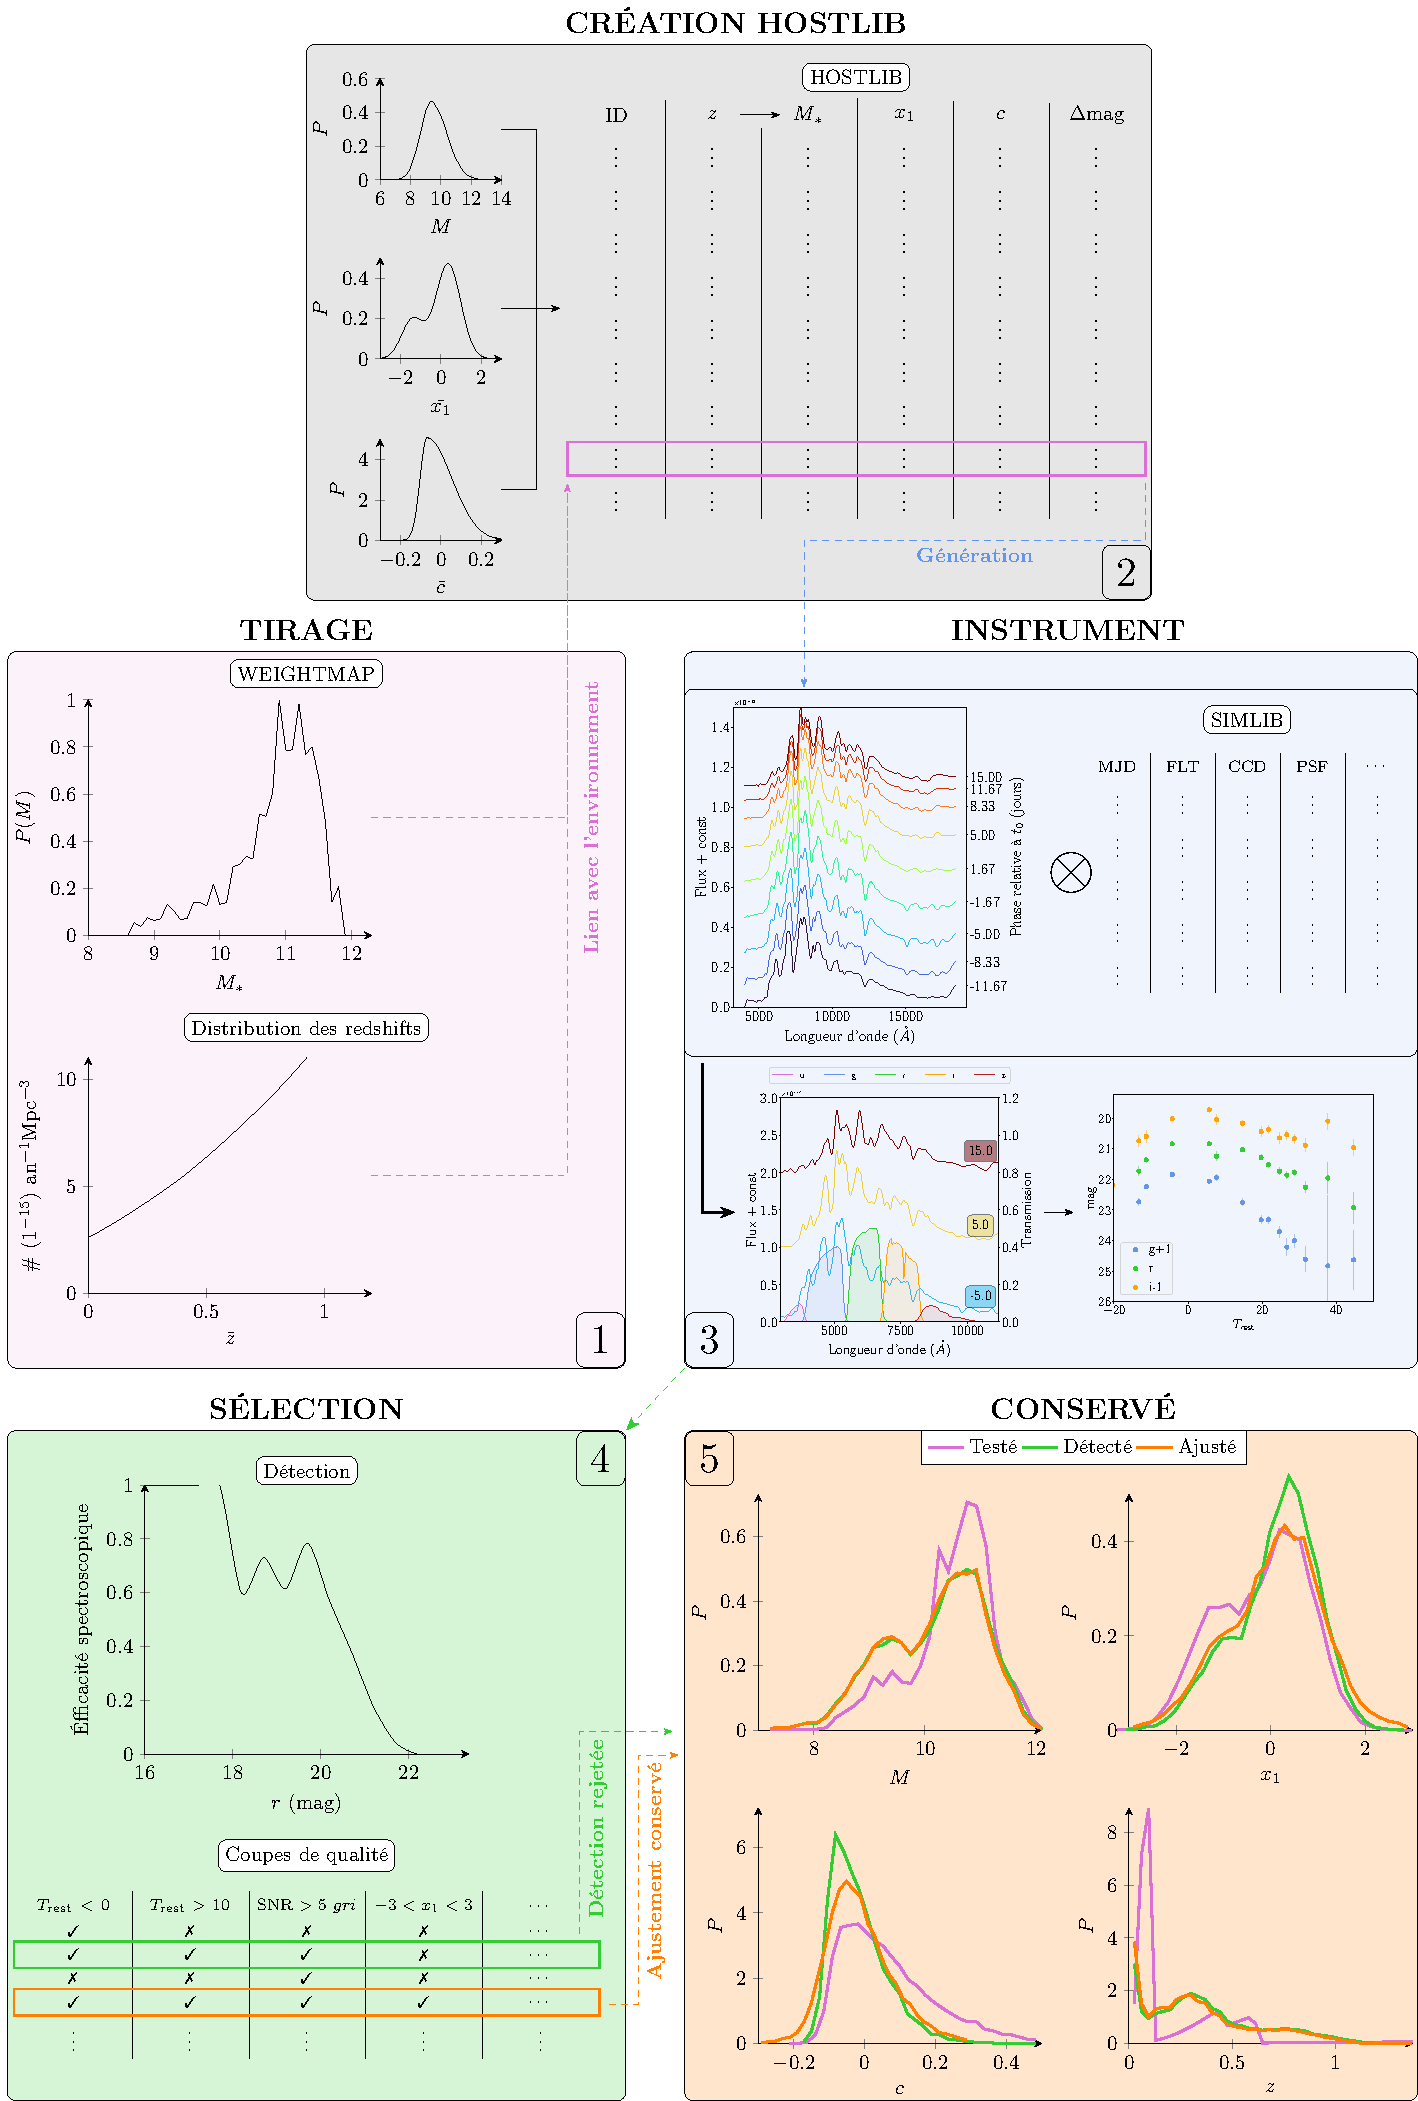
\includegraphics[width=1\linewidth]{snana_layout}
    \caption[Schéma de fonctionnement d'une simulation avec
    \snana]{\footnotesize Les tables de \wgtmap, \simlib, et de l'efficacité
        spectroscopique sont des données, ici celles du sondage SDSS. En amont
        de la simulation, une \hostlib\ est créée (\textit{en gris}, «~Création
        \hostlib~»). Pour simuler une SN~Ia, un redshift est sélectionné depuis
        une distribution (étape 1 \textit{en rose}, partie «Tirage») et est
        relié à un environnement \textit{via} un tirage la \hostlib\ pondérée
        par une carte de poids (étape 2 \textit{en gris}). À ce tirage sont
        reliées les valeurs de $x_1$ et $c$ permettant de générer une série
        temporelle de SN. Une simulation d'observation est effectuée en y
        appliquant les paramètres simulés du télescope d'un sondage grâce à une
        \simlib, donnant une courbe de lumière théorique (étape 3 \textit{en
        bleu}, partie «~Instrument~»). Cette courbe de lumière doit ensuite
        passer les critères de détection et de qualité (étape 4 \textit{en
        vert}, partie «~Sélection~»), et pourra alors être ajustée et conservée
        (orange) ou non (vert). Nous indiquons \textit{en orange} (étape 5,
        partie «~Conservé~») et pour chaque étape de ce procédé l'évolution des
        distributions de masse, étirement, couleur et redshift d'une de nos
    simulations. L'analyse se trouve Chapitre~\ref{ch:sims}}
    \label{fig:snana_func}
\end{figure}

% SNANA is a combination of tools to simulate SNe Ia data and exploit these to put
% constraints on cosmological parameters by fitting a Hubble diagram with them.
% There are 3 main parts to this procedure: (1) generate a lightcurve by modeling
% a SN and how each survey would acquire it, taking selection effects into
% account; (2) fit said lightcurve with \texttt{SALT2.4} and extract the ; (3) infer distance modulus values using bias
% correction.
% 
% The simulation inputs include a rest-frame source model, volumetric rate
% versus redshift, cosmological parameters (e.g., $\Omega_M$ , w), telescope
% transmission in each passband, calibration reference, observing and image
% properties from a survey, and random numbers to generate Poisson fluctuations.
% The simulated light curves are treated like calibrated light curves from a
% survey, and are thus analyzed with the same software as for the data.
% 
% The heart of this framework is a set of two libraries. First, an observation
% library where each observation date includes a characterization of the point
% spread function (PSF), sky and readout noise, template noise, zero point, and
% gain. Second, a host-galaxy library includes magnitudes and surface profiles,
% and is used to compute Poisson noise and to model the local surface brightness.
% For a specified light curve model, these libraries are used to convert
% top-of-the-atmosphere model magnitudes into observed fluxes and uncertainties.
% After a survey has completed, assembling the li
% 
% These tools begin by generating a Spectral Energy Distribution to which are
% applied astrophyical effects such as lensing, dimming, redshifting or galactic
% extinction, giving a first simulated magnitude. Then this magnitude is converted
% into an observed one (flux) by reproducing the effects of the instruments: zero
% point, sky noise and PSF. Selection effects are finally applied to mimick the
% triggering of which events are analyzed; these include the needed number of
% detections and needed band(s) and the spectroscopic efficiency function of the
% simulated surveys. This leads to simulated lightcurves, and after a

\section{Correction de biais et cosmologie}\label{sec:biais}
\subsection{Présentation}\label{ssec:bbcintro}

Dans cette section nous présentons l'étape d'ajusteur de cosmologie avec
corrections des biais de \snana\ basé sur la méthode \textit{BEAMS with Bias
Correction} \citep[\bbc,][]{kessler2017}. BEAMS est l'acronyme de
\textit{Bayesian Estimation Applied to Multiple Species} (estimation bayésienne
appliquée à de multiples espèces), une méthode d'ajusteur établie
dans~\cite{kunz2007} visant à prendre en compte de manière réaliste la
contamination de données non-Ia dans celles des SNe~Ia qui affects l'étude de la
cosmologie avec les SNe~Ia. Dans notre cas, nous ne simulons pas de SNe non-Ia
et ignorons les termes de vraisemblances qui y sont reliés.

Comme introduit dans la Section~\ref{ssec:simsn}, sans biais de mesure le module
de distance de la SN simulée serait $\mu_{\rm vrai}$ de
l'Équation~\ref{eq:mutrue}, et un ajustement du diagramme de \textsc{Hubble}
avec ces valeurs ne redonnerait que la cosmologie d'entrée. Avec les valeurs de
$m_b$, $x_1$, $c$ et les caractéristiques de l'environnement de l'ajustement par
\texttt{SALT2.4} qui aura passé les étapes précédentes, un ajustement du
diagramme de \textsc{Hubble} pourrait donner un décalage à ce modèle, mais reste
sous-optimal étant donné que les biais de sélection et d'ajustement de courbes
de lumière ne sont pas pris en compte. L'intérêt de \bbc\ est d'inclure la
mesure de ces biais dans le calcul du module de distance~; ainsi la SN se voit
attribuée un module de distance selon le cadre de la méthode \bbc, définit dans
\citep{popovic2021a}~:
\begin{equation}\label{eq:mu}
    \mu = m_B + \alpha x_1 - \beta c - M_{z_i} + \delta\mu_\mathrm{host} +
    \delta\mu _\mathrm{biais}
\end{equation}

La méthode d'ajustement utilisée par \bbc\ se base sur
la méthode \texttt{SALT2mu} de~\cite{marriner2011}, qui permet d'ajuster
$\alpha$ et $\beta$ sans ajustement conjoint des paramètres cosmologiques~:
ceux-ci sont d'abord fixés, puis le programme définit des intervalles de
redshifts suffisamment petits pour considérer qu'à l'intérieur de ceux-ci les
SNe~Ia sont indépendantes de la cosmologie. À leurs valeurs de module de
distance est soustrait la cosmologie de référence, donnant un décalage du module
de distance $\Delta_{\mu,z}$ dans de multiples intervalles de redshifts.
L'ajustement des valeurs de $\alpha$ et $\beta$ se fait alors à cette étape, et
l'extraction des paramètres cosmologiques s'obtient ensuite en ajustant le
module de distance (ou son décalage) avec le redshift, selon le modèle et ses
limites de paramètres («~priors~»). Cela permet de varier la cosmologie
sous-jacente sans répéter l'ajustement des $\alpha$ et $\beta$.

Ainsi, $M_{z_i}$ est l'écart de distance dans l'intervalle de redshift $z_i$,
tel que $\mu = \mu_{\rm vrai}$ lorsque les valeurs initiales de $m_b$, $x_1$ et
$c$ de la partie Génération (Section~\ref{ssec:simsn}) sont entrées à la place
des valeurs ajustées dans l'Équation~\ref{eq:mu}.

$\delta\mu_{\rm host}$ est le biais sur la luminosité selon l'environnement de
la SN, dans notre cas une marche de magnitude basée sur la masse («~mass step~»)
ou basée sur l'âge («~age step~»), de la forme
\begin{equation}
    \delta\mu_{\rm host} = \gamma\times \left( 1 + e^{X_{\rm stellar}-S}
    \right)^{-1} - \frac{\gamma}{2}
\end{equation}
avec $\gamma$ l'amplitude de la différence magnitude entre les SNe~Ia dont
l'hôte est massif ($M_* > 10^{10}\si{\Msun}$) ou non ($M_* < 10^{10}\si{\Msun}$)
pour la \textit{mass step} ou entre les SNe~Ia vieilles ou jeunes pour la
\textit{age step}. Le logiciel ne permettant pas encore d'utiliser l'âge comme
traceur, cette implémentation du biais dû à l'âge de l'environnement n'est pas
représentative de la réalité~; nous en discutons au chapitre suivant.

Finalement, $\delta\mu_{\rm bias}$ est la correction au module de distance. Il
existe différentes manières de mesurer ce biais selon les variables avec
lesquelles il est calculé, que nous présentons dans les sections suivantes.

\subsection{BBC1D}\label{ssec:bbc1D}

Originellement, il est calculé selon une seule dimension, le redshift. On
appelle cette implémentation BBC1D. Elle se base sur des intervalles de redshift

% generation of fluxes
% from a source model, application of noise, and detec-
% tion based on a characterisation of the difference imag-
% ing pipeline and/or spectroscopic selection. The simu-
% lation generates a rest-frame SED for each SNIa epoch
% and applies a combination of cosmological effects (such as
% dimming and redshift) and galactic effects (weak lensing, 
% peculiar velocity, galactic extinction). Next, the SED is
% integrated for each filter to determine broadband fluxes.
% Poisson noise is computed from the sky noise, source flux,
% PSF, and zero point. Finally, the simulation checks de-
% tections, applies the survey-dependent candidate logic,
% and applies a model for spectroscopic identification effi-
% ciency.

% \section{Introduction}
% \textit{General talk about SNe Ia, Hubble diagram, constraints and assumptions
% from BBC to fit HD.}
% 
% With that goal in mind, some recent studies try to improve the known
% correlations. In \textbf{NR21}, we presented an initial study of the drift of
% the underlying SNe~Ia stretch distribution as the function of redshift. We based
% this study on the assumption of two populations of SNe~Ia, young and old, and
% implemented different modelings of their distributions to better represent the
% observed data. For that end we took SNe~Ia data and created a complete sample by
% applying redshift cuts corresponding to the expected distance where no selection
% effects should impact each survey. This approach was at the time the simplest
% one to implement but does not allow to ponder the impact such a modeling has on
% the cosmology, and mainly on $w$, and skips all selection effects altogether.
% 
% Other studies tend to define and refine other correlations between a SN's
% brightness and some observable properties, such as their host-galaxy's mass
% (\textbf{Sullivan10, Betoule14, Smith20}) or Star Formation Rate
% (\textbf{Uddin17, Kim18, Rigault20}). One of the most common ways to test these
% correlations is to use simulations (\textbf{Kessler09a, Scolnic18, Brout19}).
% The SuperNova ANAlysis package (\snana, \textbf{Kessler09b}) allows to simulate
% surveys by using underlying distributions of parameters and correlations between
% them with the aim to find which ones come closest to the actual data.
% \textbf{Scolnic \& Kessler 16} describes the procedure of finding these
% distributions, implementing accurate selection effects for each survey, noise
% and intrinsic scatter that shift them to the observed distributions. In this
% framework, it's a galaxy's stellar mass ($M_\mathrm{stellar}$) that is assumed
% as the main observable responsible for its environmental effects on SNe~Ia. The
% goal is to correct the values of SNe affected by Malmquist bias by computing the
% average of the simulated ones, as opposed to our first approach of getting rid
% of the affected SNe.
% 
% These simulated surveys have been used to study the dependence with redshift of
% the bias correction (\textbf{Kessler 09a, Betoule14}), but showed remnant
% correlations in the computed distance moduli (SK16). The analysis thus went from
% 1-dimensional to a 5-dimensional parameter space, studying the correlations with
% redshift, color, stretch, color-luminosity and stretch-luminosity relationship
% parameters ($\alpha$, $\beta$) as developed by \textbf{Kessler \& Scolnic 17}
% with the BEAMS with Bias Corrections (BBC) method, hereafter refered to as
% BBC5D. This method is used in both the Dark Energy Survey 3 years (DES3YR,
% \textbf{Abbott19, Brout19b}) and Panoramic Survey Telescope and Rapid Response
% System (PAN-STARRS, \textbf{Scolnic18, Jones18}) analyses. This formalism was
% further improved based on the work of \textbf{Smith20}


% SK16 is galaxy distribution from which you draw, P21 is a list with the
% distrubtion already in it, linking the relationships and $x_1$ and stuff
% already drawn. But there's no evolution in it, and we want to do that. Forward
% model that through.

% General, Brodie, us; no lightcurve fitting, and at the end of hostlib section
% w simulate antheon

% P21: There is a relationship, we'll try to guess it. Take data bns of mass,
% and calculate what the distribtion of stretch is for each. Looks differently
% in different bins: as a function of mass they have distribution. Backward
% models.  N21: our data is independent and we use it to show that it works on
% other data at higher redshift, is predictive, and involves an evolution of the
% distributions.

% Generate $z$, take closest $M$ entry in a table of host galaxies (HOSTLIB),
% then pick $x_1$, $c$ assuming underlying relationships defined by the BBC
% team.  Because we want to make these simulations with an evolving underlying
% distribution, we have to replace then $x_1$ values by what is estimated by our
% previous model.

% Section 3

% Having mass isn't constitutive of SNANA, not a requirment, but we use it
% because the actual data we compare our simulated data to is described using
% mass. So we need a link betwwen LsSFR to mass: high-redshift galaxies only
% have mass measurments, not LsSFR. Quote Martin's paper.

% given model and observation strategy, what do you see like SIMSURVEY.

% SImulation part of SNANA separate from distance.

\clearpage

\thispagestyle{plain}
% \vspace*{-3cm}
\vfill
\minilof
\vfill
\minilot
\vfill

\clearpage

\appsec{Présentation des fichiers}{sec:snanainputs}

\bibliographystyle{../main/aa_url}
\shorthandoff{:}
\bibliography{../chapters/99_references}

\end{document}
